\section{Modelización la volatilidad}
Tipos de volatilidad:
\begin{itemize}
    \item \textbf{Actual volatility}: Es la medida de la cantidad de aleatoriedad en el retorno de un activo en un instante dado, variando de momento a momento sin asociarse a una escala temporal.
    \item \textbf{Historical or realized volatility}: Es una medida de la aleatoriedad en un periodo pasado específico, calculada con métodos matemáticos y utilizada como estimación para la volatilidad futura.
    \item \textbf{Implied volatility}: Es la volatilidad que, al ser introducida en el modelo de Black-Scholes, iguala el precio de mercado de la opción, reflejando la expectativa del mercado sobre la volatilidad futura. Se ha introducido en la sección~\ref{sec:vol_imp}.
    \item \textbf{Forward volatility}: Es la volatilidad asociada a un periodo de tiempo futuro o a un instante futuro, ya sea actual o implícita.
\end{itemize}



\subsection{Volatilidad por media estadística}

\subsubsection{Volatilidad constante}
Para el caso de volatilidad constante o variaciones lentas, entonces se puede considerar:
\[
\boxed{\sigma^2 = \frac{1}{N} \sum_{i=1}^{N} R_i^2}
\]
donde 
\[
R_i = \frac{S_i - S_{i-1}}{S_{i-1}}
\]
representa el retorno del día $i$. Este método tiene limitaciones, como el efecto espurio que hace que por picos instantáneos muy altos o muy bajos, la volatilidad se mantendrá muy alta durante unos días.


\subsubsection{Volatilidad con regresión a la media}
Considerando una volatilidad dependiente del tiempo y para modelar que la volatilidad tiende a una media a largo plazo $\overline{\sigma}$, se usa el modelo \textbf{ARCH (Autoregressive Conditional Heteroscedasticity)} asigna un peso a cada estimación de volatilidad a largo plazo y a la estimación actual basada en los últimos $n$ retornos:
\[
\boxed{\sigma_n^2 = \alpha \overline{\sigma}^2 + (1 - \alpha) \frac{1}{n} \sum_{i=1}^{n} R_i^2}
\]
Donde $\alpha$ es el parámetro que controla la importancia relativa entre la volatilidad a largo plazo y la volatilidad basada en los retornos recientes.



\subsubsection{Volatilidad con media móvil exponencialmente ponderada (EWMA)}
Se utiliza el modelo:
\[
\sigma_n^2 = (1 - \lambda) \sum_{i=1}^{\infty} \lambda^{i-1} R_{n-i+1}^2
\]
donde $\lambda$ es un parámetro entre 0 y 1 que controla el peso de los retornos pasados. Este modelo asigna mayor peso a los retornos más recientes. La expresión puede simplificarse como:
\[
\boxed{\sigma_n^2 = \lambda \sigma_{n-1}^2 + (1 - \lambda) R_n^2}
\]
Esto utiliza el retorno más reciente y la estimación previa de la volatilidad, siendo conocido como la medida de volatilidad de RiskMetrics.


\subsubsection{Modelo GARCH}
El modelo GARCH (Generalized Autoregressive Conditional Heteroscedasticity) combina la volatilidad a largo plazo, la volatilidad previa y los retornos recientes para estimar la volatilidad actual:
\[
\boxed{\sigma_n^2 = \alpha \overline{\sigma}^2 + (1 - \alpha) \left( \lambda \sigma_{n-1}^2 + (1 - \lambda) R_n^2 \right)}
\]
Este modelo es útil para capturar la dinámica de la volatilidad en el tiempo, considerando tanto la persistencia como la regresión hacia una media a largo plazo.

\subsubsection{Volatilidad futura esperada}
Estando a día $n$ se quiere estimar la volatilidad en $k$ días, i.e.\ en el día $n+k$. Dos maneras de hacerlo son:
\begin{itemize}
    \item Modelo \textbf{EWMA}:
    \begin{align*}
        \sigma_{n+k}^2 &= \lambda \sigma_{n+k-1}^2 + (1 - \lambda) R_{n+k}^2 \Rightarrow \\
        \Rightarrow \mathbb{E}[\sigma_{n+k}^2] &= \lambda \mathbb{E}[\sigma_{n+k-1}^2] + (1 - \lambda) \mathbb{E}[R_{n+k}^2] \Rightarrow \\
        \Rightarrow \mathbb{E}[\sigma_{n+k}^2] &= \lambda \mathbb{E}[\sigma_{n+k-1}^2] + (1 - \lambda) \mathbb{E}[\sigma_{n+k}^2]
    \end{align*}
    luego
    \[
    \boxed{\mathbb{E}[\sigma_{n+k}^2] = \mathbb{E}[\sigma_{n+k-1}^2]}
    \]
    Esto implica que la volatilidad futura esperada es igual a la estimación de volatilidad del día anterior.
    \item Modelo \textbf{GARCH}:
    \begin{align*}
        \sigma_{n+k}^2 &= \alpha \overline{\sigma}^2 + (1 - \alpha) \left( \lambda \sigma_{n+k-1}^2 + (1 - \lambda) R_{n+k}^2 \right) \Rightarrow \\
        \Rightarrow \mathbb{E}[\sigma_{n+k}^2] &= \alpha \overline{\sigma}^2 + (1 - \alpha) \left( \lambda \mathbb{E}[\sigma_{n+k-1}^2] + (1 - \lambda) \mathbb{E}[R_{n+k}^2] \right) \Rightarrow\\
        \Rightarrow \mathbb{E}[\sigma_{n+k}^2] &= \frac{\alpha \overline{\sigma}^2}{1 - (1 - \alpha)(1 - \lambda)} + \frac{\lambda (1 - \alpha)}{1 - (1 - \alpha)(1 - \lambda)} \mathbb{E}[\sigma_{n+k-1}^2]
    \end{align*}
    Mirando más hacia el futuro:
    \[
    \boxed{\mathbb{E}[\sigma_{n+k}^2] = \overline{\sigma}^2 + \left( \mathbb{E}[\sigma_{n}^2] - \overline{\sigma}^2 \right) (1 - \nu)^k} \text{ , } \qquad \nu = \frac{\alpha}{1 - (1 - \alpha)(1 - \lambda)}
    \]
\end{itemize}


\begin{figure}[H]
    \centering
    \begin{subfigure}[b]{0.45\linewidth}
        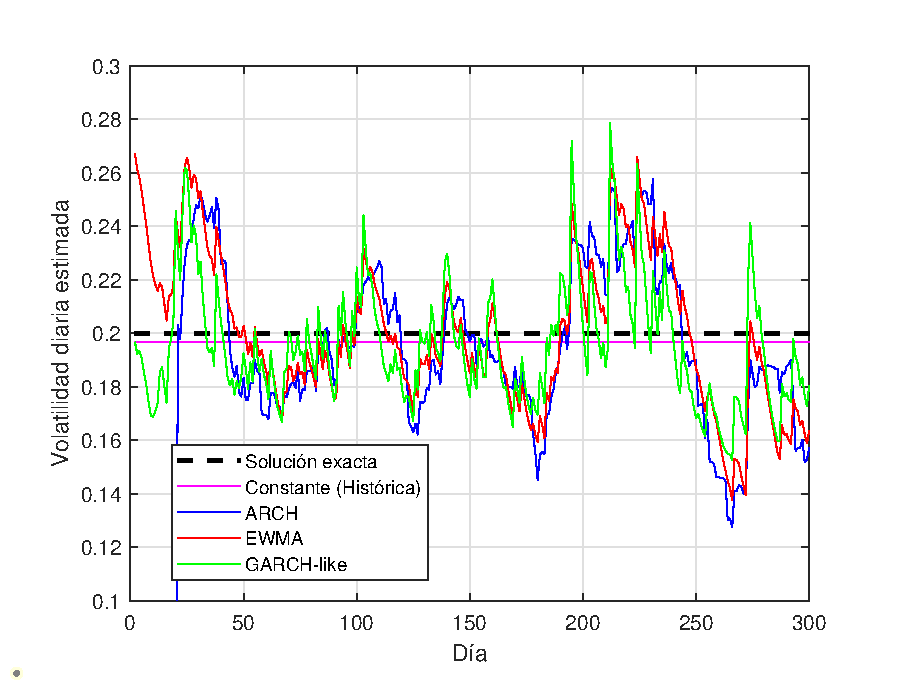
\includegraphics[width=\linewidth]{Imagenes/7_Volatilidad/Volatilidad.eps}
    \end{subfigure}
    \begin{subfigure}[b]{0.5\linewidth}
        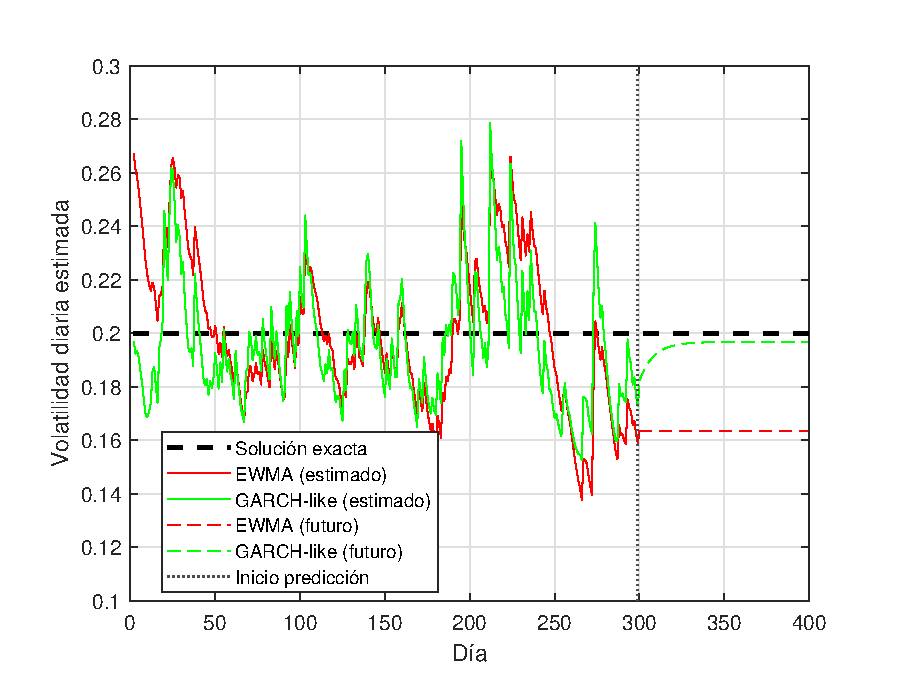
\includegraphics[width=\linewidth]{Imagenes/7_Volatilidad/Volatilidad_Prediccion.eps}
    \end{subfigure}
    \begin{subfigure}[b]{0.45\linewidth}
        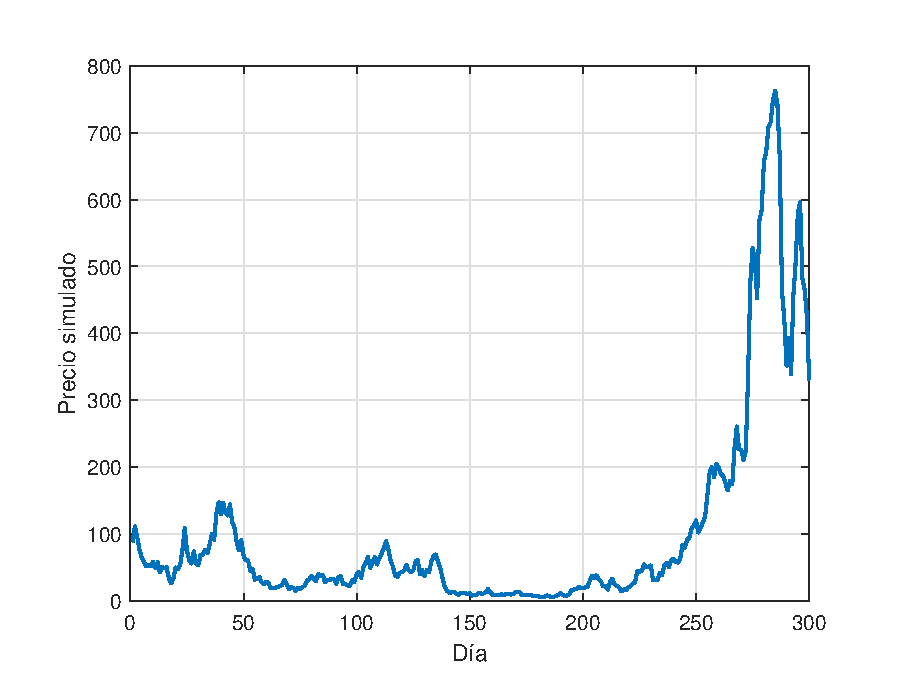
\includegraphics[width=\linewidth]{Imagenes/7_Volatilidad/Accion.eps}
    \end{subfigure}
    \caption{Comparación de estimadores de volatilidad}
\end{figure}



\subsubsection{Estimación de volatilidad basada en rangos de tiempo}
Usar demasiados datos puede capturar variaciones temporales del parámetro, mientras que usar pocos datos puede generar errores de muestreo. En primer lugar, sabiendo que \textit{Varianza\_anual = Varianza\_diaria $\times$ Número\_días\_trading}, entonces la volatilidad anualizada sería:
\[
\boxed{\sigma_{anual} = \sigma_{diaria} \times \sqrt{\textit{Número\_días\_trading}}}
\]
Algunas maneras de estimar la volatilidad diaria según los rangos de tiempo son:
\begin{itemize}
    \item \textbf{Medición tradicional close-to-close}: Sea $C_i$ el precio de cierre del día $i$, entonces:
    \begin{itemize}
        \item \textbf{Drift pequeño}:
        \[
        \boxed{\sigma^2_{cc} = \frac{1}{n} \sum_{i=1}^{n} \left( \log \left( \frac{C_i}{C_{i-1}} \right) \right)^2}
        \]
        \item \textbf{Drift genérico}:
        \[
        \boxed{\sigma^2_{acc} = \frac{1}{n-1} \sum_{i=1}^{n} \left( \left( \log \left( \frac{C_i}{C_{i-1}} \right) \right)^2 - \frac{\left( \log \left( \frac{C_n}{C_0} \right) \right)^2}{n(n-1)} \right)}
        \]
    \end{itemize}
    \item \textbf{Medición basada en rangos extremos (Parkinson, 1980)}: Utiliza los valores extremos del día, los máximos $H_i$ y los mínimos $L_i$. Es 5 veces más efectiva que la medición close-to-close:
    \[
    \boxed{\sigma_p^2 = \frac{1}{4n \log(2)} \sum_{i=1}^{n} \left( \log \left( \frac{H_i}{L_i} \right) \right)^2}
    \]

    \item \textbf{Medición basada en rangos extremos y apertura (Garman \& Klass, 1980)}: Utiliza los valores extremos del día y el precio de apertura $O_i$. Es 7.4 veces más efectiva que la medición close-to-close:
    \[
    \boxed{\sigma_{gk}^2 = \frac{1}{n} \sum_{i=1}^{n} \left( 0.511 \left( \log \left( \frac{H_i}{L_i} \right) \right)^2 - 0.019 \log \left( \frac{C_i}{O_i} \right) - 2 \log \left( \frac{H_i}{O_i} \right) \log \left( \frac{L_i}{O_i} \right) \right)}
    \]

    \item \textbf{Medición basada en rangos extremos y cierre (Rogers \& Satchell, 1991)}: Es independiente del drift, no como Parkinson y Garman \& Klass:
    \[
    \boxed{\sigma_{rs}^2 = \frac{1}{n} \sum_{i=1}^{n} \left( \log \left( \frac{H_i}{C_i} \right) \log \left( \frac{H_i}{O_i} \right) + \log \left( \frac{L_i}{C_i} \right) \log \left( \frac{L_i}{O_i} \right) \right)}
    \]
\end{itemize}





\subsection{Estimar parámetros: maximum likelihood estimation (MLE)}
Llegas a una ciudad y coges el taxi número 20922, ¿cuantos taxis hay en la ciudad? El concepto del MLE consiste en elegir los parámetros de manera que se maximice la probabilidad de que ocurra el evento observado. En este caso, la probabilidad de subirse en un taxi en específico es de $1/N$ y el $N$ que maximiza la probabilidad de subirse en el taxi 20922 es $N=20922$ $(100\%)$.

La lógica es la siguiente: se tiene un modelo (p.e.\ una normal de media 0 y desviación a estimar) con 3 (o los que sean) parámetros (p.e.\ desviación). Obtengo varios datos, calculo su probabilidad de ocurrir para cada uno de los modelos, hago una probabilidad conjunta de todos los datos y se elige el modelo que maximice esa probabilidad conjunta.

Matemáticamente, el proceso es el siguiente, sabiendo que para una distribución normal con media cero y desviación estándar $\sigma$, la probabilidad de obtener un valor $\phi_i$ es:
\[
\frac{1}{\sqrt{2\pi}\sigma} e^{-\frac{\phi_i^2}{2\sigma^2}}
\]
Luego la probabilidad conjunta de obtener $N$ valores $\phi_1, \phi_2, \dots, \phi_N$ es:
\[
\prod_{i=1}^N \frac{1}{\sqrt{2\pi}\sigma} e^{-\frac{\phi_i^2}{2\sigma^2}}
\]
Para maximizar esta probabilidad conjunta, se deriva con respecto a $\sigma$:
\begin{align*}
    &\frac{\partial}{\partial \sigma} \left( \prod_{i=1}^N \frac{1}{\sqrt{2\pi}\sigma} \exp\left(-\frac{\phi_i^2}{2\sigma^2}\right) \right) = 0 \Rightarrow \\
    \Rightarrow &\frac{\partial}{\partial \sigma} \left( \left( \frac{1}{\sqrt{2\pi}\sigma} \right)^N \exp\left(-\frac{1}{2\sigma^2} \sum_{i=1}^N \phi_i^2\right) \right) = 0 \Rightarrow \\
    \Rightarrow &\frac{\partial}{\partial \sigma} \left( \ln\left(\left( \frac{1}{\sqrt{2\pi}\sigma} \right)^N \exp\left(-\frac{1}{2\sigma^2} \sum_{i=1}^N \phi_i^2\right)\right) \right) = 0 \Rightarrow \\
    \Rightarrow &\frac{\partial}{\partial \sigma} \left( N\ln\left(\frac{1}{\sqrt{2\pi}\sigma}\right) - \frac{1}{2\sigma^2} \sum_{i=1}^N \phi_i^2 \right) = 0 \Rightarrow \\
    \Rightarrow &\frac{\partial}{\partial \sigma} \left( -N\ln\left(\sqrt{2\pi}\right) -N\ln\left(\sigma\right) - \frac{1}{2\sigma^2} \sum_{i=1}^N \phi_i^2 \right) = 0 \Rightarrow \\
    \Rightarrow &-\frac{N}{\sigma} + \frac{1}{\sigma^3} \sum_{i=1}^N \phi_i^2 = 0 \Rightarrow \\
    \Rightarrow &\sigma^2 = \frac{1}{N} \sum_{i=1}^N \phi_i^2
\end{align*}



